\chapter{Referencial teórico}\label{ch:referencial}

Esta seção dispõe de uma breve revisão bibliográfica de assuntos referentes ao tema do projeto, que são 
os seguintes: túneis de vento, tubos de Pitot e mesas de posicionamento. Por fim, apresenta trabalhos 
relacionados que envolvem estes assuntos.

\section{Túnel de vento}\label{sec:tunel}

Os túneis de vento são estruturas que propiciam a simulação para o desenvolvimento de estudos que relacionam 
o efeito do movimento de ar em torno de objetos, como turbinas, aviões, carros e edificações. Sua estrutura 
é composta por um duto de diâmetro adequado onde o ar é empurrado ou succionado por um ventilador. No 
interior do duto, o ar é analisado através de instrumentos de medição.

%PRECISA COLOCAR A REFERENCIA \cite{carminatti2019desenvolvimento} não achei o goreck esse cita gorek
O primeiro túnel de vento foi construído na Inglaterra em 1871 por Frank H. Wenham (1824-1908), engenheiro 
naval britânico e membro da Sociedade Aeronáutica da Grã-Bretanha, esse túnel era de circuito fechado e 
acionado por uma máquina a vapor. Os estudos de Wenham permitiram avanços no alongamento de uma asa 
relacionado à força de sustentação \cite{carminatti2019desenvolvimento}.

%PRECISA COLOCAR A REFERENCIA \cite{joglekar2014design}
Em 1897 foi construído por Konstantin Tsiolkovsky o primeiro túnel de vento Russo que era de circuito 
aberto com um ventilador centrífugo e determinou os coeficientes de arrasto de placas planas, cilindros 
e esferas \cite{joglekar2014design}. 

%PRECISA COLOCAR A REFERENCIA \cite{de2014adalberto}
Devido às guerras, a produção de túneis de vento teve uma demanda aumentada, pois era necessário a execução 
de ensaios em aeronaves militares. Já após o período de guerras, os túneis de vento ganharam relevância 
quando o objetivo foi aumentar a eficiência na aerodinâmica dos carros \cite{de2014adalberto}. 

%PRECISA COLOCAR A REFERENCIA \cite{pritchard2005fox}
Os túneis de vento podem ser classificados quanto ao circuito que pode ser aberto ou fechado, quanto a velocidade 
de escoamento em relação à velocidade do som que é chamada de número de Mach (Ma) definindo os escoamentos como sônico, 
subsônico, supersônico e hipersônico e quanto ao sentido do escoamento que nos túneis de vento de circuito aberto podem 
ser soprador e sugador, sendo definido pela condição de trabalho do ventilador \cite{pritchard2005fox}.

O túnel de vento tratado neste trabalho está situado junto ao Laboratório de Sistemas Térmicos da Universidade Federal 
do Rio Grande e é de característica subsônica, circuito aberto e do tipo soprador.

\section{Tubo de Pitot}\label{sec:tubo}

O tubo de Pitot foi um equipamento criado por Henri Pitot em 1732 para medição da vazão do rio Sena. 
Pitot de maneira intuitiva apresentou que a altura de uma coluna de líquido conectada ao seu tubo era 
proporcional à raiz quadrada da velocidade. Ele desenvolveu a técnica mais comum para determinação 
da velocidade de um fluido, pois a utilização desse tubo é simplificada, além do baixo custo.

O tubo de Pitot apresenta vantagens como sua flexibilidade na utilização de diferentes faixas de velocidade 
desde o regime subsônico ou supersônico, sendo possível a obtenção de velocidades com alta precisão. 
No entanto apresenta desvantagens de falta de precisão em baixas velocidade, impossibilidade de medição 
em escoamentos reversos e dificuldade de obtenção de medições em alta frequência.

%PRECISA COLOCAR A REFERENCIA \cite{pritchard2005fox}
Com essa técnica, Pitot obteve a velocidade em um escoamento incompressível em uma área pontual, sendo que 
é necessário o tubo ser posicionado de modo a ficar alinhado com o escoamento. Com isso se mede a pressão 
estática e a pressão total ou de estagnação. A subtração da pressão total da estática resulta na pressão 
dinâmica do escoamento \cite{pritchard2005fox}.

\begin{figure}[!htb]
\centering
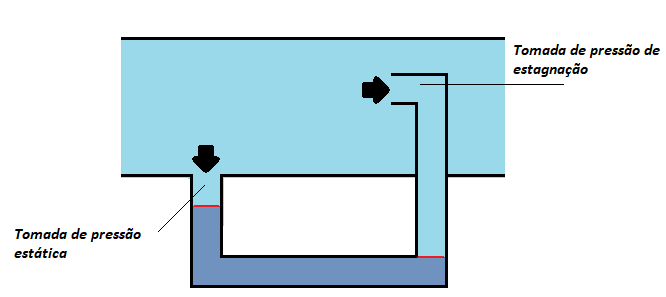
\includegraphics[scale = 0.7]{figuras/pestagnacao}
\caption{Funcionamento das pressões dentro do tubo de Pitot.}
\caption*{Fonte: Próprio autor.}
\label{fig:pestagnacao}
\end{figure}

%PRECISA COLOCAR A REFERENCIA \cite{pritchard2005fox}
Seu princípio de funcionamento está baseado na conhecida equação de Bernoulli onde 
a pressão dinâmica ($p_{d}$) é igual a pressão total ($p_{t}$) menos a pressão estática ($p_{e}$) \cite{pritchard2005fox}.

\begin{equation}\label{eq:pdinamica}
    pd = pt - pe
\end{equation}
\begin{equation}\label{eq:bernoulli}
    \frac{p_{1}}{\rho} + \frac{1}{2} \cdot (V_{1})^{2} + g \cdot z_{1} = \frac{p_{2}}{\rho} + \frac{1}{2} \cdot (V_{2})^{2} + g \cdot z_{2} = cte  
\end{equation}
\begin{equation}\label{eq:binicial}
    p_{e} + \frac{1}{2} \cdot \rho \cdot (V)^{2} + \rho \cdot g \cdot z_{e} = p_{t} + \frac{1}{2} \cdot \rho \cdot (0)^{2} + \rho \cdot g \cdot z_{t} = cte  
\end{equation}
\begin{equation}\label{eq:velocidade}
    V = \sqrt{\frac{2 \cdot (p_{t} - p_{e})}{\rho}}
\end{equation}
\begin{equation}\label{eq:roar}
    \rho_{ar} = \frac{P_{atm}}{R_{ar} \cdot T_{ar}}
\end{equation}

Sendo que $p_{1}$ é a pressão estática no ponto 1, $V_{1}$ é a velocidade do fluído no ponto 1, $\rho$ 
é a massa específica do fluido, $g$ é a força gravitacional e $p_{2}$ é a pressão total.

% ARRUMAR SIMBOLOS
A equação \ref{eq:velocidade} serve para obter a velocidade a partir da pressão e é obtida 
através da equação de Bernoulli para regime permanente, incompressível e sem atrito 
conforme a equação \ref{eq:bernoulli}. Percebe-se que a massa específica é função da condição 
de estado do ar durante os testes sendo determinada a partir da Equação \ref{eq:roar}. 
Onde $R_{ar}$ é e $T_{ar}$ é...

\section{Mesa de posicionamento}\label{sec:mesa}

Utilizada para várias finalidades como, posicionamento de peças que serão usinadas em máquinas de Controle 
Numérico Computadorizada (CNC’s), automação de laboratórios, armazenamento de cargas, impressões 3D entre 
outros tantos propósitos, as mesas cartesianas tem como função principal o posicionamento de alguma 
ferramenta, para executar algum tipo de serviço.

% PRECISA COLOCAR A REFERENCIA Figura 2.2 e Figura 2.3
Também conhecidas como mesa de posicionamento XY, pois como o nome sugere, é uma estrutura com dois eixos 
de liberdade que permite o posicionamento da peça ou da ferramenta em algum lugar de um plano pré-definido. 
Podem ser classificadas em dois tipos com relação a sua transmissão: as mesas acionadas por fusos conforme 
apresenta a Figura \ref{fig:mfuso} e as acionadas por correias sincronizadas demonstradas na Figura \ref{fig:mcorreia}.

%PRECISA COLOCAR A REFERENCIA \cite{rocha2015retrofitting} \cite{kassouf2003mesa} não encontrei o kassouf
As mesas de posicionamentos de fuso possuem um alto rendimento, próximo de 95\%, um baixo desgaste e uma 
velocidade máxima de 3 m/s, já as mesas acionadas por correias sincronizadas podem desenvolver velocidades 
de até 5 m/s, conseguindo altas acelerações devido a sua inércia \cite{rocha2015retrofitting}.

\begin{figure}[!htb]
\centering
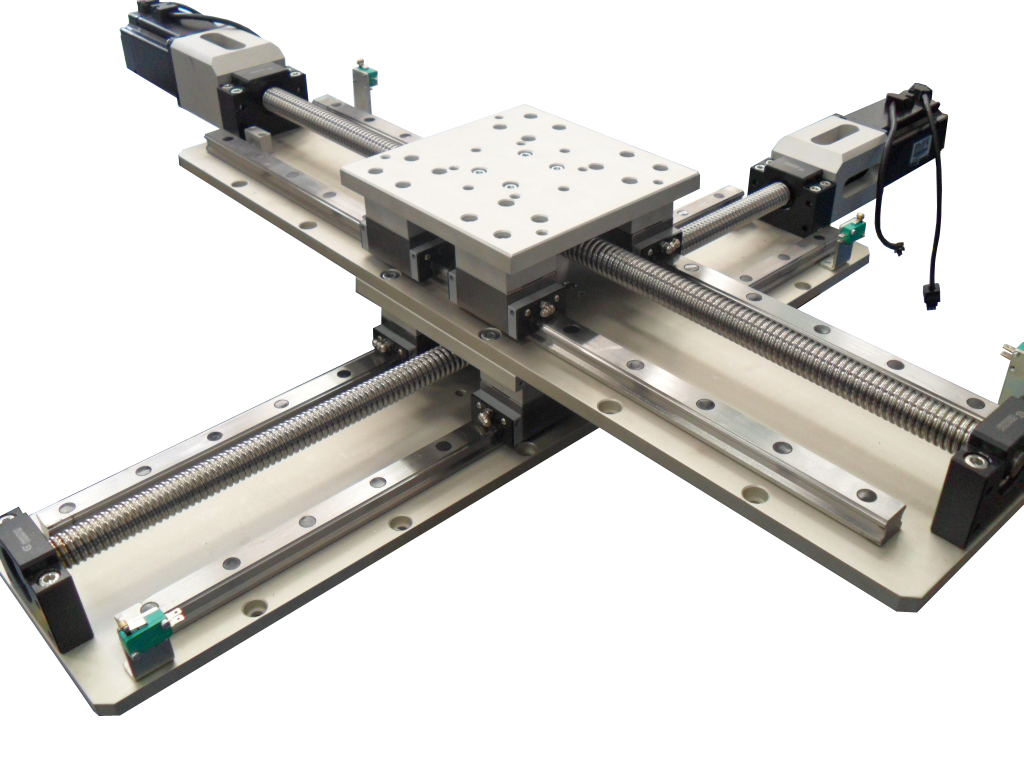
\includegraphics[scale = 0.3]{figuras/mfuso}
\caption{Mesa acionada por fuso.}
\caption*{Fonte: https://www.kalatec.com.br/mesa-de-coordenada-xy/}
\label{fig:mfuso}
\end{figure}
    
\begin{figure}[!htb]
\centering
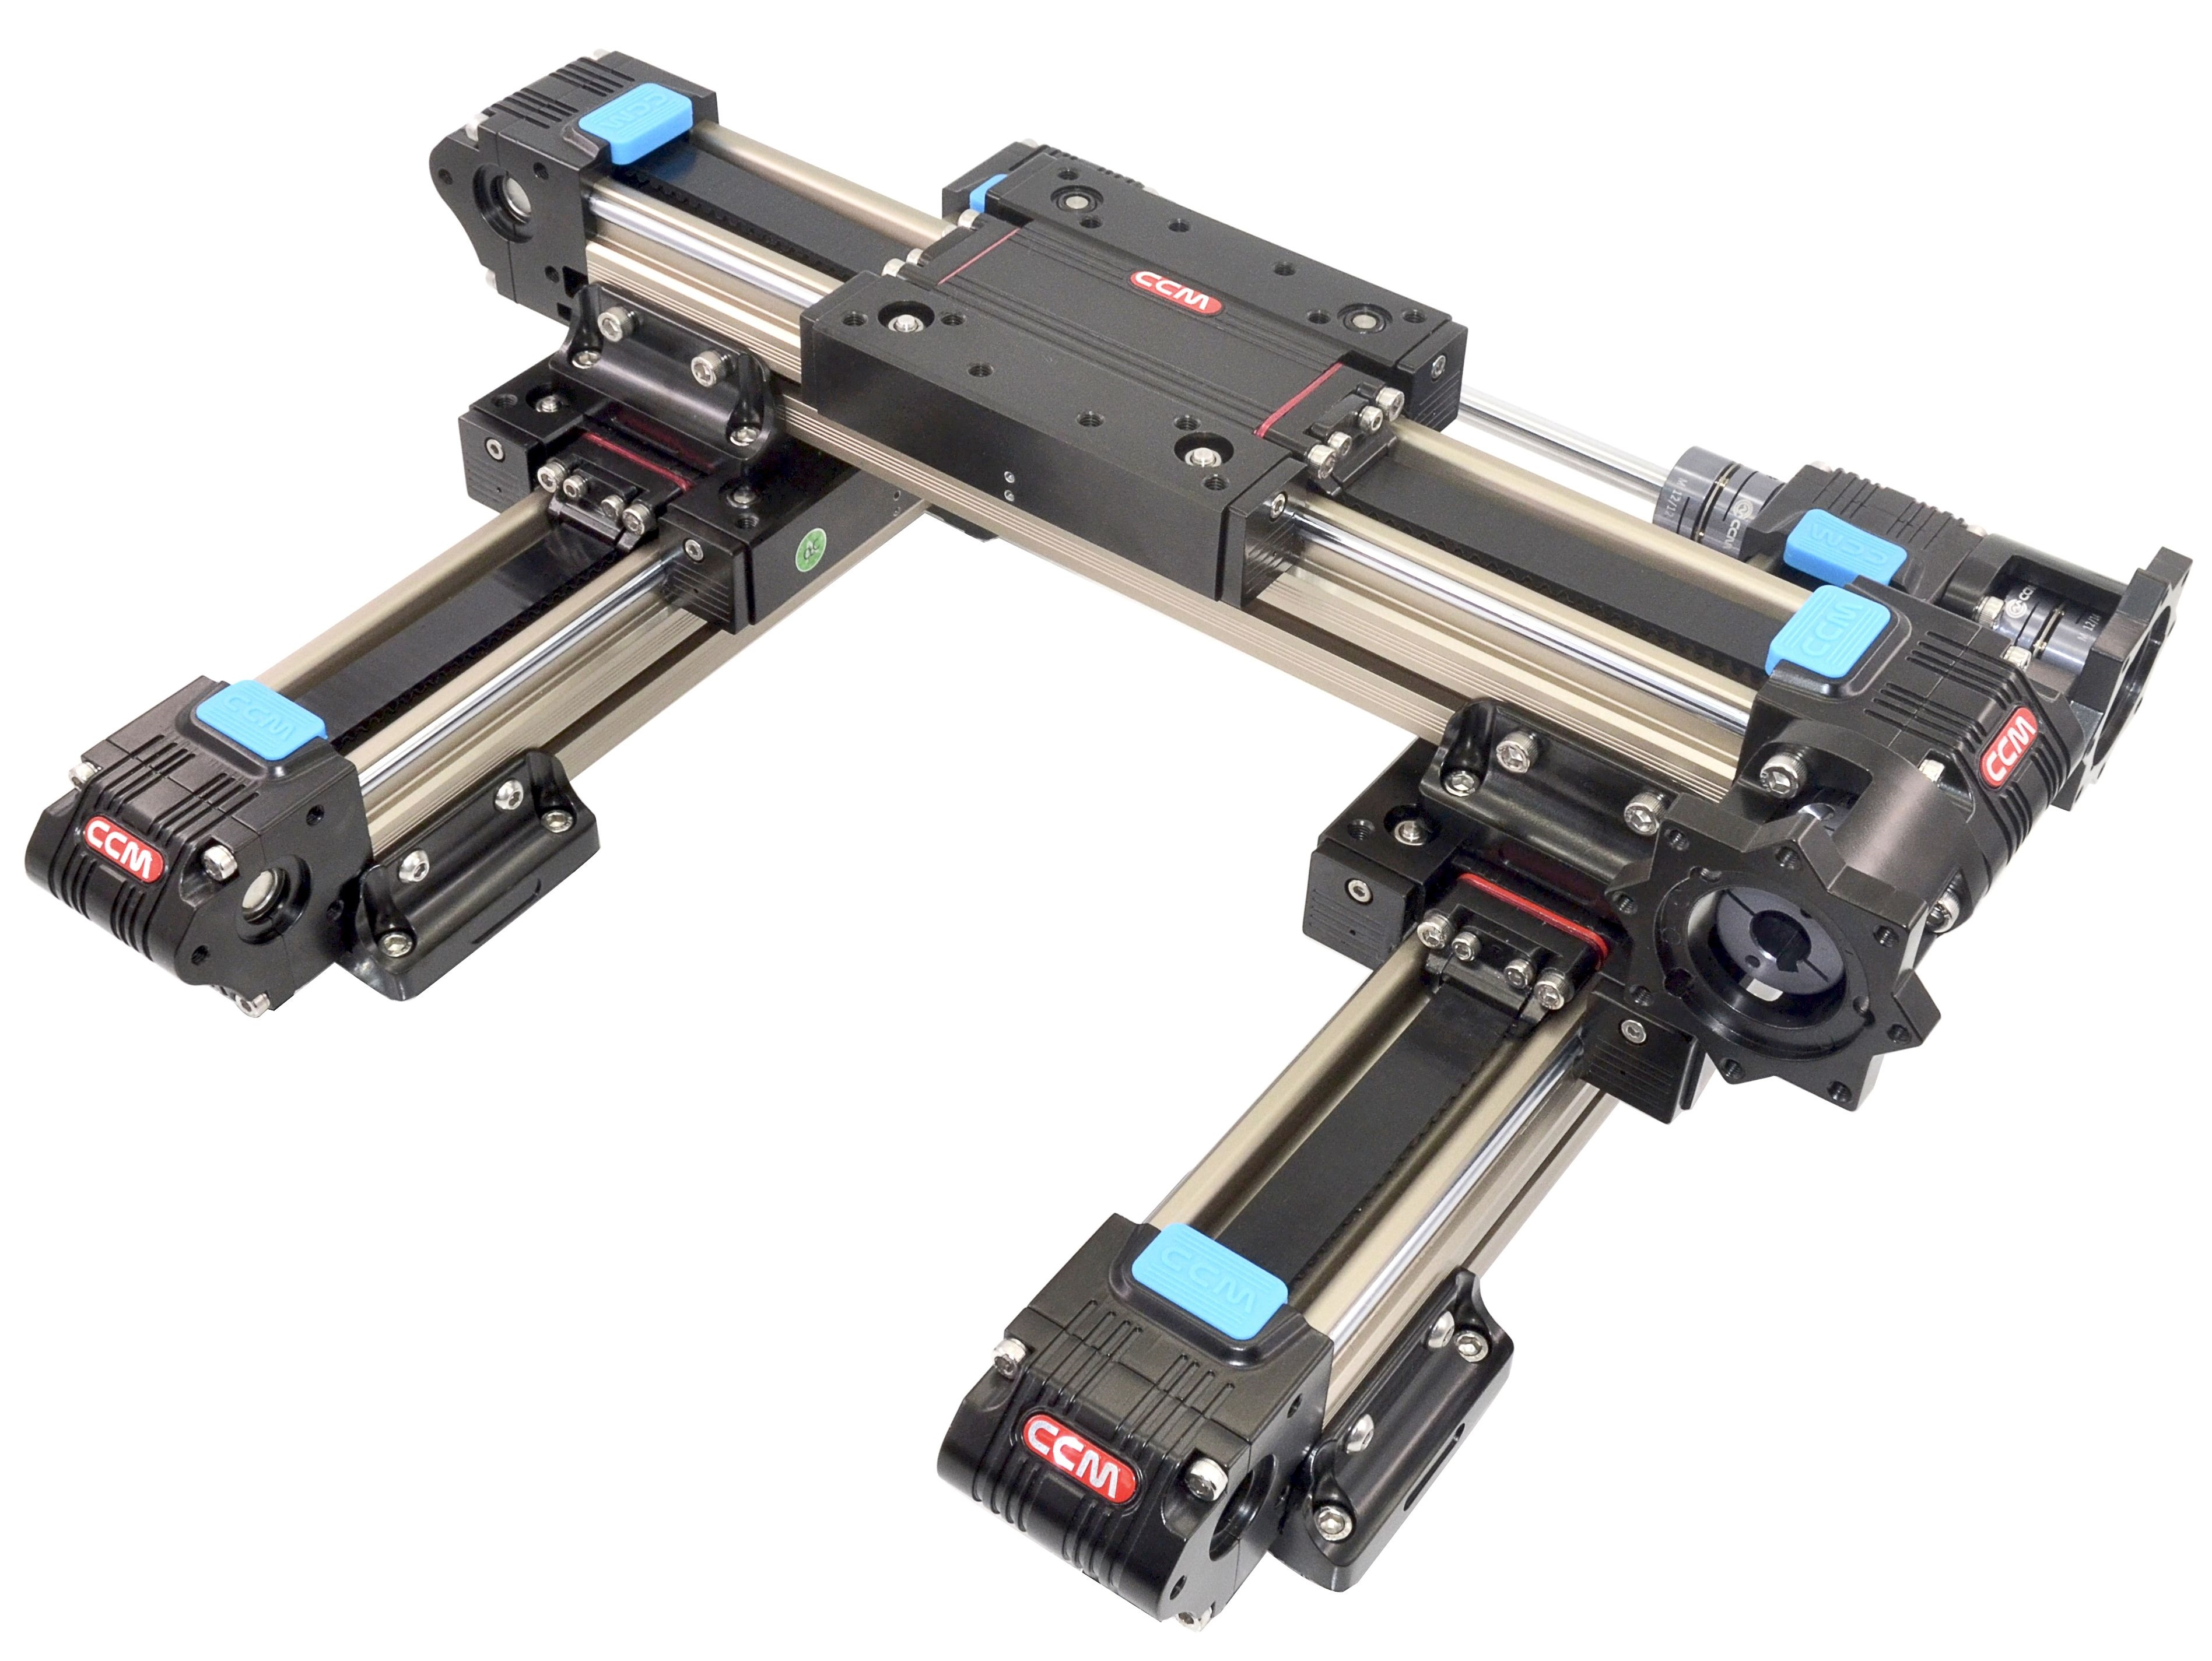
\includegraphics[scale = 0.065]{figuras/mcorreia}
\caption{Mesa acionada por correias.}
\caption*{Fonte: https://www.ccmrails.com/2019/01/26/packing-automation/}
\label{fig:mcorreia}
\end{figure}
    
%PRECISA COLOCAR A REFERENCIA não encontrei
Outro componente importante nesse mecanismo é o acionador, que pode ser um motor de passo ou um servomotor. 
Os motores de passo são máquinas que exercem um papel muito importante atualmente, são utilizados em 
aplicações onde é requerido um alto grau de precisão no movimento e que este movimento seja feito em passos 
fixos, referentes a uma fração de ângulo. Empregados normalmente quando se deseja controlar uma combinação 
entre a posição do rotor (ângulo), com a devida velocidade e o sincronismo \cite{silva2018maquinas}.

O funcionamento desse motor se dá através dos princípios do eletromagnetismo, com estatores bobinados e um rotor 
formado por ímãs permanentes ligados ao eixo. Quando o estator é energizado cria um campo magnético e o rotor 
move-se para alinhar os ímãs (pólos norte e sul) com as linhas de fluxo magnético, formados pelo estator, 
movendo o eixo em um ângulo pequeno chamado de passo e continua a girar conforme o incremento angular controlado 
por circuitos eletrônicos. Esses circuitos digitais tem como função repassar a informação, um pulso, recebido 
pelo sistema de controle para o motor, que gira com grande precisão conforme seu controle. Como característica 
marcante, os motores com ímãs permanentes apresentam um torque estático quando não submetidos à tensão devido 
a força magnética entre os ímãs e o estator, servindo como freio para o sistema.
 
\section{Trabalhos relacionados}\label{sec:trabalhos}

Nesta seção serão apresentados trabalhos relacionados ao tema deste projeto apresentando os objetivos e resultados 
de cada um.

%PRECISA COLOCAR A REFERENCIA \cite{butignol2017adequaccao}
O trabalho realizado por \citeauthor{butignol2017adequaccao} (\citeyear{butignol2017adequaccao}), 
tinha o objetivo de desenvolver uma adequação de uma mesa XYZ didática acionada por motores 
de passo para o estudo de programação em em microcontroladores e seu posicionamento em duas dimensões.

%PRECISA COLOCAR A REFERENCIA \cite{butignol2017adequaccao}
Como resultado do trabalho, \citeauthor{butignol2017adequaccao} (\citeyear{butignol2017adequaccao}) 
desenvolveu um aparato eletromecânico de posicionamento de dois eixos e um atuador no terceiro eixo 
capaz de auxiliar no ensino de microcontroladores. Por fim, o projeto está disponível 
em~<https://mesaxydidatica.blogspot.com.br> para sua montagem em outras instituições de ensino.

%PRECISA COLOCAR A REFERENCIA \cite{camargo1988mesa}
O trabalho realizado por \citeauthor{camargo1988mesa} (\citeyear{camargo1988mesa}), tinha o objetivo de 
desenvolver um sistema posicionador de baixo custo com \acrfull{CNC}, utilizando componentes 
nacionalizados e com uma complexidade mínima no sistema de comando.

Como resultado do trabalho, \citeauthor{camargo1988mesa} (\citeyear{camargo1988mesa}) fez uma análise 
comparando diversos parâmetros como: massa, frequência natural amortecida, amplitude média da curva de 
resposta, perdas de passo, erros de posicionamento, vibração entre outros a fim de demonstrar que a 
concepção projetada e executada para a mesa de coordenadas XY presente em seu estudo, se 
justifica com os resultados obtidos.

%PRECISA COLOCAR A REFERENCIA \cite{ramos2018desenvolvimento}
O trabalho realizado por \citeauthor{ramos2018desenvolvimento} (\citeyear{ramos2018desenvolvimento}), 
tinha o objetivo de projetar e construir uma mesa cartesiana para ser colocada nos túneis 
aerodinâmicos existentes no Departamento de Engenharia Mecânica e Industrial da Faculdade de Ciências e 
Tecnologia Universidade Nova de Lisboa, para assim, dar a capacidade de deslocamento de sensores como: tubo de Pitot, 
anemômetro de fio quente, anemômetro laser-Doppler para qualquer ponto na seção escolhida.

%PRECISA COLOCAR A REFERENCIA \cite{ramos2018desenvolvimento}
Como resultado do trabalho, \citeauthor{ramos2018desenvolvimento} (\citeyear{ramos2018desenvolvimento}) construiu 
uma mesa cartesiana funcional com capacidade de efetuar medições de velocidade em uma malha de cem posições, 
podendo inserir coordenadas através da porta serial do Arduino. Ainda comprovou por testes experimentais a 
precisão dos motores de passo ao comprovar que não existe diferença mensurável entre o valores medidos com os ideais.

%PRECISA COLOCAR A REFERENCIA \cite{hoss2018implantaccao}
O trabalho realizado por \citeauthor{hoss2018implantaccao} (\citeyear{hoss2018implantaccao}), tinha o objetivo 
a instrumentação e desenvolvimento do sistema de controle de velocidade do vento de um túnel de vento com 
propulsão por motor a combustão interna, existente no laboratório de Conformação do IFSC Campus Chapecó.

%PRECISA COLOCAR A REFERENCIA \cite{hoss2018implantaccao}
Como resultado do trabalho, \citeauthor{hoss2018implantaccao} (\citeyear{hoss2018implantaccao}) alcançou o objetivo 
permitindo medir variáveis de forma confiável com incertezas pequenas dentro dos requisitos estabelecidos, mesmo 
com emprego de sensores de baixo custo e média precisão.
